\documentclass{standalone}
\usepackage{pgfplots}
\pgfplotsset{compat=1.13}

\begin{document}

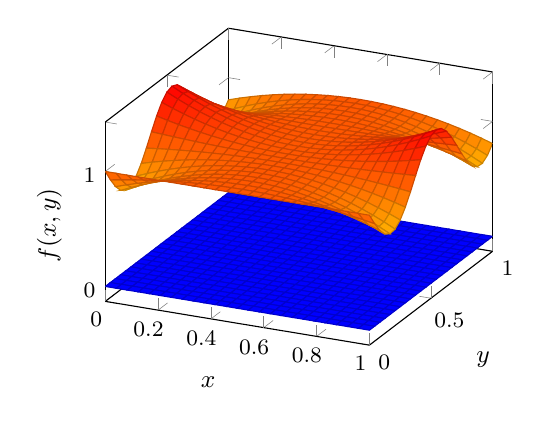
\begin{tikzpicture}
    \begin{axis}[
            xlabel={$x$}, ylabel={$y$}, zlabel={$f(x,y)$},
            xmin = 0, xmax = 1, ymin = 0, ymax = 1,
            small,
        ]
        \addplot3[
            surf,
            domain=0:1,
            domain y=0:1,
        ]{0};
        \addplot3[
            surf,
            domain=0:1,
            domain y=0:1,
        ]{1 - 1.2* (x-.5)*(x-.5)*sin(500*y)};
    \end{axis}
\end{tikzpicture}

\end{document}